\documentclass[tikz]{standalone}
\begin{document}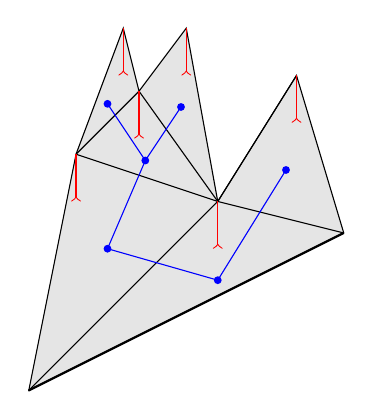
\begin{tikzpicture}[scale=2]
\coordinate (x0) at (0,0);
\coordinate (x1) at (2,1);
\coordinate (x2) at (1.7,2);
\coordinate (x3) at (1.2,1.2);
\coordinate (x4) at (1,2.3);
\coordinate (x5) at (.7,1.9);
\coordinate (x6) at (.6,2.3);
\coordinate (x7) at (.3,1.5);

\coordinate (t0) at (barycentric cs:x0=2,x1=3,x3=1);
\coordinate (t1) at (barycentric cs:x1=1,x2=1,x3=1);
\coordinate (t2) at (barycentric cs:x0=1,x3=1,x7=1);
\coordinate (t3) at (barycentric cs:x3=2,x5=1,x7=2);
\coordinate (t4) at (barycentric cs:x3=1,x4=1,x5=1);
\coordinate (t5) at (barycentric cs:x4=1,x6=1,x7=3);

\filldraw[draw=black,fill=gray!20] (x0) -- (x1) -- (x2) -- (x3) -- (x4) -- (x5) -- (x6) -- (x7) -- (x0) -- cycle;
\draw[thick] (x0) -- (x1);
\draw (x0) -- (x3);
\draw (x1) -- (x3);
\draw (x3) -- (x7);
\draw (x3) -- (x5);
\draw (x3) -- (x2);
\draw (x7) -- (x5);

\foreach \i in {2,3,4,5,6,7}
\draw[red,-<] (x\i) -- +(0,-.3);

\foreach \i in {0,1,2,3,4,5}
\node[circle,fill,blue,inner sep=1pt] at (t\i) {};

\draw[blue] (t0) -- (t1);
\draw[blue] (t0) -- (t2) -- (t3) -- (t4);
\draw[blue] (t3) -- (t5);


\end{tikzpicture}\end{document}
